\chapter{Compiling OpenQASM using MLIR}
% draw a diagram of the compilation pipeline

\begin{figure}[ht]
    \centering
    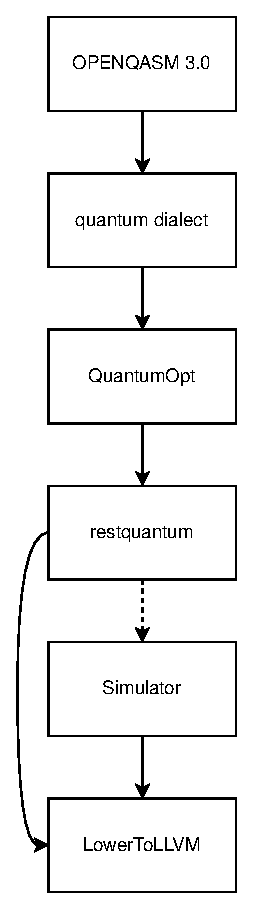
\includegraphics{images/pipeline.eps}
    \caption[caption]{Compilation Pipeline Stages}
    \medskip
    \small
    Note: the dotted line is to show that the quantum simulator
    is an optional lowering step and can be circumvented when deploying on
    real quantum hardware.
    \label{fig:compilation_pipeline}

\end{figure}

\section{Overview}
\label{sec:overview}
OPENQASM 3.0 compilation goes through a few phases. The first one being the
frontend compilation phase. Namely, the OPENQASM 3.0 code is parsed and
converted into a concrete syntax tree (CST), using ANTLR4 parser generator, to a
c++ runtime target. The CST is traversed using the visitor pattern through
generated visitor methods. These methods are then overridden to generate MLIR
code. Generation of MLIR code for classical OPENQASM 3.0 instructions is quite
straight forward, it is done using MLIR built-in dialects. However, for quantum
instructions, we created our own quantum dialect, named \texttt{quantum},
introducing types for qubits, and a set of quantum operations. Some quantum
optimizations are then performed on theses quantum operations, such as the
elimination of identity gates. This is then lowered to another dialect called
\texttt{restquantum}, which represents a restricted set of quantum gates. These
set of gates are the ones supported by the Walter Meiner Institute(WMI) quantum
computer, as of time of writing. This is of course not the only possible
lowering step, and can be extended to support other hardware. Now, since for the
scope of this thesis we were not able to test our code on the WMI quantum
computer, we created a quantum simulator written purely in MLIR, which can be
used to test our code. Therefore, the next step for our compilation pipeline is
to convert operations of
the \texttt{restquantum} dialect to other built-in MLIR dialects. Finally, we
lower all the MLIR code to LLVM IR, and then to machine code by LLVM's
Just-In-Time (JIT) compiler, to be executed.
An overview of the stages of the pipeline are shown in Figure \ref{fig:compilation_pipeline}.

\section{Dialects Created}
The quantum dialect has been created to represent quantum operations, and
qubits. Both types and operations are opaque. This means that they don't have an
inherent interpretation and can be lowered dependent on the target quantum
hardware or simulator.  Some operations and types are shared between the two dialects.
The class diagram for the two dialects are shown in Figures \ref{fig:quantum_dialect} and \ref{fig:restquantum_dialect}.
In the next two subsections we will describe the operations and types created in each dialect.
\subsection{Quantum Dialect}
The main types created are:
\begin{itemize}
    \item \texttt{quantum.Array} - represents a quantum register, which is a
          collection of qubits.
    \item \texttt{quantum.Qubit} - represents a qubit, which is a quantum bit.
\end{itemize}
Both of these types are also used in the \texttt{restquantum} dialect.
% set width of figure
\begin{figure}
    \centering
    \includegraphics[width=\textwidth]{images/quantum_dialect.pdf}
    \caption[Quantum Dialect]{Class diagram of quantum dialect}
    \label {fig:quantum_dialect}
\end{figure}
The main operations created are:
\begin{itemize}
    \item \texttt{quantum.qalloc} - allocates a quantum register of size
          \texttt{size}.
    \item \texttt{quantum.dealloc} - frees a quantum register.
    \item \texttt{quantum.qextract} - extracts a qubit from a quantum register,
          at index \texttt{index}.
    \item \texttt{quantum.mz} - measures a qubit in the standard basis.
    \item \texttt{quantum.print\_global\_vector} this is a utility function to
          print the global quantum state vector in our simulator.
    \item \texttt{quantum.SingleSimpleGate} - A class representing a single
          non-parametrized qubit gate. This is reused to create many other gates.
    \item \texttt{quantum.RotationGate} - A class representing a single qubit
          gate, parametrized with an angle operand. This is reused to create other
          rotation gates.
    \item \texttt{quantum.cx} - represents a controlled x gate.
    \item \texttt{quantum.gen\_gate} - represents a generic gate, that takes in
          an arbitrary number of qubits, and arbitrary number of parameters.
\end{itemize}
\subsection{RestQuantum Dialect}
\begin{figure}
    \centering
    \includegraphics[width=\textwidth]{images/restquantum_dialect.pdf}
    \caption[Quantum Dialect]{Class diagram of restquantum dialect}
    \label {fig:restquantum_dialect}
\end{figure}
The \texttt{restquantum} dialect is a restricted set of quantum gates, which
are supported by the WMI quantum computer. All these gates, except for the iSWAP gate,
perform a rotation around an axis in the Bloch sphere, at certain angles.
These gates are:
\begin{itemize}
    \item \texttt{restquantum.rx90} - represents a rotation around the x axis by
          90 degrees.
    \item \texttt{restquantum.rx180} - represents a rotation around the x axis
          by 180 degrees - equivalent to a Pauli X gate up to a global phase.
    \item \texttt{restquantum.ry90} - represents a rotation around the y axis by
          90 degrees.
    \item \texttt{restquantum.ry180} - represents a rotation around the y axis
          by 180 degrees - equivalent to a Pauli Y gate up to a global phase.
    \item \texttt{restquantum.rz90} - represents a rotation around the z axis by
          90 degrees.
    \item \texttt{restquantum.rz180} - represents a rotation around the z axis
          by 180 degrees - equivalent to a Pauli Z gate up to a global phase.
    \item \texttt{restquantum.sqrtx} - represents a square root of the Pauli X
          gate.
    \item \texttt{restquantum.iSWAP} - represents an iSWAP gate.
\end{itemize}


\section{Pipeline}
\subsection{Frontend}
Using the ANTLR4 grammar live spec (now stable) on OPENQSM 3.0's website we
created a parser for a subset of OPENQASM 3.0. This subset can certainly be
extended to fully support the language, but for the scope of this thesis we
focused mainly on quantum gates, quantum measurement, some control flow
operations - namely if statements and while loops -, some arithmetic (bitwise or
otherwise) operations, logical operations, and main type declarations(quantum or
classical). To do this lowering we used ANTLR's parser generator JAR file, which
generated a c++, tokenizer(\texttt{qasmLexer}) and parser(\texttt{qasmParser}),
along with a visitor class(\texttt{qasmBaseVisitor}) having methods for each of
the grammar rules. We then overrode these methods in the class \texttt{Visitor}
to generate MLIR code. The parsing starts by passing an input \texttt{.qasm}
file to the \texttt{MLIRGenerator} class, which then tokenizes it with ANTLR's
generated tokenizer, and parses the tokens with ANTLR's generated parser.
Starting at the start rule of OPENQASM 3.0's grammar (which is
\texttt{program}), the visitor traverse the CST and builds MLIR code upon
visiting nodes of supported OPENQASM 3.0 constructs.
\subsection{Translation to MLIR}
To first inialize MLIR code building, we first need to create an
\texttt{MLIRContext} pointer, and load all the desired dialects in the MLIR code
building. This can be done as follows:
\begin{minted}{c++}
    // create an MLIR context pointer 
    auto context = std::make_unique<MLIRContext>();

    // load quantum dialect 
    context->loadDialect<quantum::QuantumDialect();

    // load restquantum dialect
    context->loadDialect<restquantum::RestrictedQuantumDialect>();
    
    // load vector dialect
    context->loadDialect<vector::VectorDialect>();

    // load arithmetic dialect 
    context->loadDialect<arith::ArithDialect>();

    // ...etc
\end{minted}

Next we initialize an Operation Builder, of class \texttt{OpBuilder}, which is
used to build MLIR operations. We pass a source code (.qasm) location to the
\texttt{ModuleOp} builder, to construct a module operation, which is the root of
the MLIR code. We finally construct a \texttt{FuncOp} of name \texttt{main} with
no arguments, and an Integer 64 (I64) return type, and append it to the module
operation. This is an analogue to the main function in C/C++, and is the entry
point of the MLIR code. We set this function to be the operation builder's
insertion point, to ensure that created operation are appended to the function.
After all OPENQASM to MLIR translations are done, we build a final
\texttt{ReturnOp} operation with an \texttt{arith::ConstantOp} of value 0, and
append it to the function. In the next sections we will discuss different
compiler passes we applied to transform our MLIR code. Compiler passes are
essentially traversal of an application's Directed Acyclic Graph (DAG), and
applying a set of transformations to the graph.

\subsection{Optimization}
\label{sec:optimization}
In this thesis optimization wasn't a main focus, but we did implement simple
quantum optimization using quantum gate identities. These were only applied to
the \texttt{quantum} dialect, and not the \texttt{restquantum} dialect. To do
this we first defined our rewriter patterns simply in a TableGen file
(\texttt{Optimize.td}). The defined patterns included the following identities:
% draw a diagram of the quantum identities
% ....

These patterns are defined in the \texttt{Optimize.td} file as follows:
\begin{minted}{c++}
    // RZ(theta1) RZ(theta2) -> RZ(theta1 + theta2) 
    def RzRz: Pat<(RzOp (RzOp $input, $theta2), $theta1), 
        (RzOp $input, (Arith_AddFOp $theta1, $theta2,
        (createFastMathNone)))>;

    // HYH -> Y 
    def HYH: Pat<(HOp (YOp (HOp $input))), (YOp $input)>;

    // HZH -> Z 
    def HZH: Pat<(HOp (ZOp (HOp $input))), (ZOp $input)>;

    // HH -> I 
    def HH: Pat<(HOp (HOp $input)), (IOp $input)>;

    // ... more patterns
\end{minted}
To be able to apply these patterns in a simple manner, we employed them as parts
of MLIR's \texttt{Conanicalizer} pass. To do so we have to set the
\texttt{hasCanonicalizer} flag to 1 in the quantum dialect's definition, in its
tablegen file. Next we need to implement MLIR \texttt{Dialect}'s class override
method, \texttt{getCanonicalizationPatterns}. This is done as follows:
\begin{minted}{c++}
// #include ... 
#include "quantum-mlir/Conversion/Optimize.h.inc" 
using namespace mlir::quantum;

void QuantumDialect::getCanonicalizationPatterns(
    ::mlir::RewritePatternSet& results) const { 
        populateWithGenerated(results); 
}
\end{minted}

The \texttt{populateWithGenerated}  function defined in the generated
\texttt{Optimize.h.inc} populates \texttt{results} with the patterns defined in
\texttt{Optimize.td}. Finally, we initialize \texttt{MLIR}'s pass manager, and
add MLIR's \texttt{Canonicalizer} pass to it. We also add the \texttt{DCE} pass,
which is a dead code elimination pass, and common subexpression elimination (CSE)
pass.
The DCE pass is essential as the rewrite patterns
defined in TableGen syntax only rewrites the last quantum gate (in direction of
the quantum circuit), but leaves the remaining gates. By passing the
\texttt{NoMemoryEffect} trait to our quantum gates, we allow MLIR's \texttt{DCE}
pass to remove these remaining quantum gates as they are longer used by any
other upcoming operations. This setting is predicated on the assumption that
qubits have to be measured for the operations on them to be useful and not
removed, which is fine for our purposes. Moreover, this wouldn't cause issue for
entagled qubits because if either of them is measured both stay due to their
joint use in a CNOT gate. Note that using Canoincalizer pass here is  as it is
more intended for canonicalization of syntax, however since optimization isn't
the main goal of this thesis, this was a quick and simple way to test our idea,
but in the future this should be refactored into its own pass.


\subsection{Lowering to Restricted Quantum}
\begin{figure}
    \begin{quantikz}
        & \gate{X} & \ctrl{1} & \qw \\
        & \qw & \targ{} & \qw
        \end{quantikz}
        =\begin{quantikz}
        & \ctrl{1} & \gate{X} & \qw \\
        & \targ{} & \gate{X} & \qw
        \end{quantikz}
    \label{fig:quantum-identities}
\end{figure}
In order to lower our code to the \texttt{restquantum} dialect, we use multiple quantum gate 
identities, some of which are shown in Figure \ref{fig:quantum-identities}.

To implement this lowering in MLIR, we create a  \texttt{LowerToRestQuantum} pass.
We add this in a \texttt{Passes.td} file where we defined all necessary passes,
including relevant passes for the quantum simulator. We define it as follows:
\begin{minted}{c++}
def LowerToRestQuantum: Pass<"lower-to-restquantum", "ModuleOp"> { 
    let summary =
        "Lower quantum dialect instructions to restrict" 
      + "quantum dialect instructions"; 
    let constructor =
        "mlir::quantum::createLowerToRestQuantumPass()"; 
    let description = [{ }];
}
\end{minted}

Then in a \texttt{Passes.h} file we declare a function
\texttt{createLowerToRestQuantumPass} as follows:

\mintinline{c++}|std::unique_ptr<OperationPass<ModuleOp>>|\\
\mintinline{c++}|createLowerToRestQuantumPass();| \\Finally, we implement the pass in a
\texttt{LowerToRestQuantum.cpp} file. There we define a
\texttt{LowerToRestQuantum} class, which inherits from
\texttt{LowerToRestQuantumBase}, a class generated by MLIR's TableGen. There we
set a \texttt{ConversionTarget} \texttt{target} object with all the quantum
dialect gates as illegal operations. We also pass rewrite pattern classes, that
we defined, to  a \texttt{RewritePatternSet} object. These rewrite pattern
classes transform all quantum gates in terms of \texttt{restquantum} gates.\\
We then call MLIR's \texttt{applyFullConversion} function, which applies all the
defined patterns to the current MLIR code, and lowers all illegal operations to
legal ones. Each of the rewriter pattern classes is defined as follows:
\begin{minted}{c++}
class ConvertQOp : public OpConversionPattern<quantum::QOp> { 
    using OpConversionPattern::OpConversionPattern; 
    LogicalResult matchAndRewrite(quantum::QOp op, 
                  PatternRewriter& rewriter) const override { 
        // Create relevant restquantum gates 
        // to match a quantum identity.
        // Use rewriter.replaceOpWithNewOp 
        // to replace the quantum gate
        // with needed operations.
        // Use rewriter.create 
        // to add remaning necessary operations.
    } 
};
\end{minted}

We finally implement the \texttt{createLowerToRestQuantumPass} function,
to inialize a \texttt{unique\_ptr}  of type \texttt{LowerToRestQuantum} and return it.
To use this pass, like we did with the \texttt{Optimize} pass, we pass it
to the \texttt{PassManager} object, and run it. We also add the \texttt{CSE} pass.

\subsection{Quantum simulator (optional) pass}
The quantum simulator pass is an optional pass that can be used to simulate the
quantum circuit. It is declared similar to the \texttt{LowerToRestQuantum} pass, and
defined in its own \texttt{QuantumSimulator.cpp} file.
However, for convenience, we created a prior pass that does a forward
declaration of all quantum allocations at the start of the MLIR code.
Then, in the quantum simulator we sum the number of allocations multiplied by their qubit size,
to get the totable number of qubits needed for a global state vector.
We initialize a state vector of $\|0_{n-1}...0_0\rangle$ where $n$ is the number of qubits.
Note, we assume the $0^{th}$ qubit is the right-most qubit in the bra-ket notation, thus
accessing the $0^{th}$ element in the first qubit array accesses the right-most qubit, and accessing
the last element in the last qubit array accesses the left-most qubit.
We use MLIR's \texttt{VectorType} to represent the state vector,
and we initialize a vector of shape $2^n \times 2$, where each element
of the vector is a 2d vector denoting a complex number, this is because
complex numbers are not supported yet as types for vector elements.
Similar to what we did in the \texttt{LowerToRestQuantum} pass, we create different
rewrite patterns to replace all quantum operations (gates, allocations, and measurements)
with classical counterparts, manipulating with the initialized global
state vector. For simulating quantum gates, instead of
doing a matrix multiplication that would
involve a lot of tensoring in the case of applying a gate to a subset of qubits.
For example if we apply a gate to the first qubit of a quantum system that can be represented by a
tensor product (non-entangled), the transformation would be as follows:
\begin{equation}
    |\psi_{n-1}\rangle \otimes \psi_{n-2}\rangle  \otimes ... |\psi_0\rangle
    \rightarrow
    I  |\psi_{n-1}\rangle \otimes I  |\psi_{n-2}\rangle  \otimes ... X  |\psi_0\rangle
\end{equation}
To avoid this excessive tensoring, we reshape our vector to a tensor in a way that we can
isolate the qubit we want to apply the gate to in its own dimension, then apply the matrix of this gate
to the element in that dimension in the reshaped tensor,
and finally reshape the tensor back to a vector of the original shape.
For the case of the two-qubit gate $iSWAP$, we just swap the phases for the 
quantum states $|01\rangle$ and $|10\rangle$, and multiply them by $i$.

% Lowering the code to the \texttt{restquantum} dialect is done by the
% \texttt{ConvertInst} pass. This pass is run after the \texttt{QuantumOpt}
% pass, which performs some optimizations on the quantum code. The lowering is
% done by matching the quantum operations with the \texttt{restquantum}
% operations. Then the \texttt{restquantum} operations are created, and the
% \textt{quantum} operations are replaced with them.

\section{Examples - MLIR generated code}
For different stages of the compilation pipeline, different MLIR code is generated.
In this section we showcase the MLIR code generated by the compiler at different stages.
We start with the following OPENQASM code:
\begin{minted}{c++}
    OPENQASM 3.0;
    qubit[2] q;
    H q[0];
    Y q[0];
    H q[0];
    X q[1];
    PRINT_GLOBAL_VECTOR();
    bit[2] c;
    c[0] = measure q[0];
    c[1] = measure q[1];
    print(c);
\end{minted}
This code declares two qubits in a qubit array identified by \texttt{q}, applies a Hadamard gate to the first qubit, a Pauli-Y gate to the first qubit,
followed by another Hadamard gate, and finally an X gate to the second qubit.
Then it prints the global state vector, and finally measures the first and second qubits, and prints the result.
Note that both \texttt{PRINT\_GLOBAL\_VECTOR} and \texttt{print} are custom functions that we defined as utility functions.
The former was defined as part of the \texttt{quantum} dialect, and the latter is an addition to OPENQASM 3.0 grammar.

\subsection{Translating to the quantum dialect}
The first stage of the compilation pipeline is translating the OPENQASM code to the \texttt{quantum} dialect, 
as it was shown earlier in the \ref{sec:overview} section, as well as in figure \ref{fig:compilation_pipeline}. 
An internal MLIR structure is built at that stage, but the corresponding IR assembly can be printed to show:
\begin{minted}{c++}
module {
  func.func @main() -> i64 {
    %0 = "quantum.qalloc"() {name = "q", offset = 0 : i32, size = 2 : i64} :
     () -> !quantum.QubitArray

    %c0_i64 = arith.constant 0 : i64
    
    %1 = "quantum.qextract"(%0, %c0_i64) : 
    (!quantum.QubitArray, i64) -> !quantum.Qubit

    %2 = "quantum.HOp"(%1) : (!quantum.Qubit) -> !quantum.Qubit

    %3 = "quantum.YOp"(%2) : (!quantum.Qubit) -> !quantum.Qubit
    
    %4 = "quantum.HOp"(%3) : (!quantum.Qubit) -> !quantum.Qubit

    %c1_i64 = arith.constant 1 : i64

    %5 = "quantum.qextract"(%0, %c1_i64) : 
    (!quantum.QubitArray, i64) -> !quantum.Qubit

    %6 = "quantum.XOp"(%5) : (!quantum.Qubit) -> !quantum.Qubit
    "quantum.print_global_vector"() : () -> ()

    %cst = arith.constant dense<false> : vector<2xi1>

    %7 = "quantum.mz"(%4) : (!quantum.Qubit) -> i1

    %c0 = arith.constant 0 : index

    %8 = vector.insertelement %7, %cst[%c0 : index] : vector<2xi1>

    %9 = "quantum.mz"(%6) : (!quantum.Qubit) -> i1

    %c1 = arith.constant 1 : index

    %10 = vector.insertelement %9, %8[%c1 : index] : vector<2xi1>

    vector.print %10 : vector<2xi1>

    %c0_i64_0 = arith.constant 0 : i64

    return %c0_i64_0 : i64
  }
}

\end{minted}
In the above code, we can see the \texttt{quantum} dialect operations that were generated from the OPENQASM code, 
along with some standard MLIR operations. 
Firstly, an MLIR module is created, and a \texttt{main} function is defined in it, which returns an integer of value 0 in
the end.
The \texttt{quantum.qalloc} operation allocates a qubit array of size 2 with identifier \texttt{q}, and assigns it to the variable \texttt{q}.
Then, the \texttt{quantum.qextract} operation extracts the first qubit from the qubit array, and assigns it to the variable \texttt{q[0]}.
Similarly, the second qubit is extracted and assigned to the variable \texttt{q[1]}.
Then, the \texttt{quantum.HOp} operation is applied to the first qubit, followed by the \texttt{quantum.YOp} operation,
and then another \texttt{quantum.HOp} operation.
The \texttt{quantum.XOp} operation is applied to the second qubit.
The \texttt{quantum.print\_global\_vector} operation prints the global state vector, as explained earlier.
The \texttt{quantum.mz} operation measures the qubit in the computational basis, and returns the result as a boolean.
The \texttt{vector.insertelement} operation inserts the result of the measurement into the vector of bits, and the \texttt{vector.print} operation, 
translated from the defined \texttt{print} function, prints the vector of bits.

\subsection{Applying Optimizations}
The next stage of the compilation pipeline is applying optimizations on the code.
This utilizes a few MLIR defined optimization passes, as well as the quantum identifies defined in the \texttt{QuantumOpt} pass,
as explained earlier in the \ref{sec:optimization} section. Here is the MLIR code after applying the optimizations:
\begin{minted}{c++}
module {
  func.func @main() -> i64 {
    %c1 = arith.constant 1 : index

    %c0 = arith.constant 0 : index

    %cst = arith.constant dense<false> : vector<2xi1>

    %c1_i64 = arith.constant 1 : i64

    %c0_i64 = arith.constant 0 : i64

    %0 = "quantum.qalloc"() {name = "q", offset = 0 : i32, size = 2 : i64} : 
    () -> !quantum.QubitArray

    %1 = "quantum.qextract"(%0, %c0_i64) : 
    (!quantum.QubitArray, i64) -> !quantum.Qubit

    %2 = "quantum.YOp"(%1) : (!quantum.Qubit) -> !quantum.Qubit

    %3 = "quantum.qextract"(%0, %c1_i64) : 
    (!quantum.QubitArray, i64) -> !quantum.Qubit

    %4 = "quantum.XOp"(%3) : (!quantum.Qubit) -> !quantum.Qubit

    "quantum.print_global_vector"() : () -> ()

    %5 = "quantum.mz"(%2) : (!quantum.Qubit) -> i1

    %6 = vector.insertelement %5, %cst[%c0 : index] : vector<2xi1>

    %7 = "quantum.mz"(%4) : (!quantum.Qubit) -> i1

    %8 = vector.insertelement %7, %6[%c1 : index] : vector<2xi1>

    vector.print %8 : vector<2xi1>

    return %c0_i64 : i64
  }
}
\end{minted}

Applying the optimizations, we can see that the \texttt{quantum.HOp} operations are removed by 
the identity $HYH \equiv Y$(up to a global phase).

\subsection{Lowering to restquantum}
In the next stage of the compilation pipeline, we lower our quantum code to the \texttt{restquantum} dialect,
per the identities defined in the figure \ref{fig:quantum-identities}.
Here is the MLIR code after lowering to \texttt{restquantum}:
\begin{minted}{c++}
module {
  func.func @main() -> i64 {
    %c1 = arith.constant 1 : index

    %c0 = arith.constant 0 : index

    %cst = arith.constant dense<false> : vector<2xi1>

    %c1_i64 = arith.constant 1 : i64

    %c0_i64 = arith.constant 0 : i64
    
    %0 = "quantum.qalloc"() {name = "q", offset = 0 : i32, size = 2 : i64} :
     () -> !quantum.QubitArray

    %1 = "quantum.qextract"(%0, %c0_i64) :
     (!quantum.QubitArray, i64) -> !quantum.Qubit

    %2 = "restquantum.ry180"(%1) : 
    (!quantum.Qubit) -> !quantum.Qubit

    %3 = "quantum.qextract"(%0, %c1_i64) : 
    (!quantum.QubitArray, i64) -> !quantum.Qubit

    %4 = "restquantum.rx180"(%3) :
     (!quantum.Qubit) -> !quantum.Qubit

    "quantum.print_global_vector"() : () -> ()
    %5 = "quantum.mz"(%2) : (!quantum.Qubit) -> i1

    %6 = vector.insertelement %5, %cst[%c0 : index] : vector<2xi1>
    
    %7 = "quantum.mz"(%4) : (!quantum.Qubit) -> i1

    %8 = vector.insertelement %7, %6[%c1 : index] : vector<2xi1>

    vector.print %8 : vector<2xi1>

    return %c0_i64 : i64
  }
}
\end{minted}

\subsection{Quantum Simulator}
The next stage of the compilation pipeline is to convert all quantum operations into
classical ones that can be executed by a quantum simulator.
Here is the MLIR code after lowering to the simulator:
\begin{minted}{c++}
module {
  func.func @main() -> i64 {
    %c1 = arith.constant 1 : index
    %c0 = arith.constant 0 : index
    %cst = arith.constant dense<false> : vector<2xi1>
    %c0_i64 = arith.constant 0 : i64
    %cst_0 = arith.constant dense
    <[1.000000e+00, 0.000000e+00, 0.000000e+00, 0.000000e+00, 
     0.000000e+00, 0.000000e+00, 0.000000e+00, 0.000000e+00]> : vector<8xf64>
    %0 = vector.shape_cast %cst_0 : vector<8xf64> to vector<4x2xf64>
    %alloc = memref.alloc() : memref<vector<4x2xf64>>
    memref.store %0, %alloc[] : memref<vector<4x2xf64>>
    %1 = memref.load %alloc[] : memref<vector<4x2xf64>>
    %2 = vector.shape_cast %1 : vector<4x2xf64> to vector<2x2x1x2xf64>
    %cst_1 = arith.constant 0.000000e+00 : f64
    %cst_2 = arith.constant -1.000000e+00 : f64
    %3 = vector.extract %2[0, 0] : vector<2x2x1x2xf64>
    %4 = vector.extract %2[0, 1] : vector<2x2x1x2xf64>
    %5 = vector.extract %4[0, 0] : vector<1x2xf64>
    %6 = vector.extract %4[0, 1] : vector<1x2xf64>
    %7 = complex.create %5, %6 : complex<f64>
    %8 = complex.create %cst_1, %cst_2 : complex<f64>
    %9 = complex.mul %7, %8 : complex<f64>
    %10 = complex.re %9 : complex<f64>
    %11 = complex.im %9 : complex<f64>
    %12 = vector.insert %10, %4 [0, 0] : f64 into vector<1x2xf64>
    %13 = vector.insert %11, %12 [0, 1] : f64 into vector<1x2xf64>
    %14 = vector.insert %13, %2 [0, 0] : 
    vector<1x2xf64> into vector<2x2x1x2xf64>
    %15 = vector.extract %3[0, 0] : vector<1x2xf64>
    %16 = vector.extract %3[0, 1] : vector<1x2xf64>
    %17 = complex.create %15, %16 : complex<f64>
    %cst_3 = arith.constant 1.000000e+00 : f64
    %18 = complex.create %cst_1, %cst_3 : complex<f64>
    %19 = complex.mul %17, %18 : complex<f64>
    %20 = complex.re %19 : complex<f64>
    %21 = complex.im %19 : complex<f64>
    %22 = vector.insert %20, %3 [0, 0] : f64 into vector<1x2xf64>
    %23 = vector.insert %21, %22 [0, 1] : f64 into vector<1x2xf64>
    %24 = vector.insert %23, %14 [0, 1] : vector<1x2xf64> into vector<2x2x1x2xf64>
    %25 = vector.extract %24[1, 0] : vector<2x2x1x2xf64>
    %26 = vector.extract %24[1, 1] : vector<2x2x1x2xf64>
    %27 = vector.extract %26[0, 0] : vector<1x2xf64>
    %28 = vector.extract %26[0, 1] : vector<1x2xf64>
    %29 = complex.create %27, %28 : complex<f64>
    %30 = complex.mul %29, %8 : complex<f64>
    %31 = complex.re %30 : complex<f64>
    %32 = complex.im %30 : complex<f64>
    %33 = vector.insert %31, %26 [0, 0] : f64 into vector<1x2xf64>
    %34 = vector.insert %32, %33 [0, 1] : f64 into vector<1x2xf64>
    %35 = vector.insert %34, %24 [1, 0] : 
    vector<1x2xf64> into vector<2x2x1x2xf64>
    %36 = vector.extract %25[0, 0] : vector<1x2xf64>
    %37 = vector.extract %25[0, 1] : vector<1x2xf64>
    %38 = complex.create %36, %37 : complex<f64>
    %39 = complex.mul %38, %18 : complex<f64>
    %40 = complex.re %39 : complex<f64>
    %41 = complex.im %39 : complex<f64>
    %42 = vector.insert %40, %25 [0, 0] : f64 into vector<1x2xf64>
    %43 = vector.insert %41, %42 [0, 1] : f64 into vector<1x2xf64>
    %44 = vector.insert %43, %35 [1, 1] : vector<1x2xf64> into vector<2x2x1x2xf64>
    %45 = vector.shape_cast %44 :
     vector<2x2x1x2xf64> to vector<4x2xf64>
    memref.store %45, %alloc[] : memref<vector<4x2xf64>>
    %46 = memref.load %alloc[] : memref<vector<4x2xf64>>
    %47 = vector.shape_cast %46 : 
    vector<4x2xf64> to vector<1x2x2x2xf64>
    %48 = vector.extract %47[0, 0] : vector<1x2x2x2xf64>
    %49 = vector.extract %47[0, 1] : vector<1x2x2x2xf64>
    %50 = vector.insert %49, %47 [0, 0] : 
    vector<2x2xf64> into vector<1x2x2x2xf64>
    %51 = vector.insert %48, %50 [0, 1] : 
    vector<2x2xf64> into vector<1x2x2x2xf64>
    %52 = vector.shape_cast %51 : vector<1x2x2x2xf64> to vector<4x2xf64>
    memref.store %52, %alloc[] : memref<vector<4x2xf64>>
    %53 = memref.load %alloc[] : memref<vector<4x2xf64>>
    vector.print %53 : vector<4x2xf64>
    %54 = memref.load %alloc[] : memref<vector<4x2xf64>>
    %55 = vector.extract %54[0, 0] : vector<4x2xf64>
    %56 = vector.extract %54[0, 1] : vector<4x2xf64>
    %57 = complex.create %55, %56 : complex<f64>
    %58 = complex.abs %57 : complex<f64>
    %59 = arith.mulf %58, %58 : f64
    %60 = arith.addf %cst_1, %59 : f64
    %61 = vector.extract %54[1, 0] : vector<4x2xf64>
    %62 = vector.extract %54[1, 1] : vector<4x2xf64>
    %63 = complex.create %61, %62 : complex<f64>
    %64 = complex.abs %63 : complex<f64>
    %65 = arith.mulf %64, %64 : f64
    %66 = arith.addf %cst_1, %65 : f64
    %67 = vector.extract %54[2, 0] : vector<4x2xf64>
    %68 = vector.extract %54[2, 1] : vector<4x2xf64>
    %69 = complex.create %67, %68 : complex<f64>
    %70 = complex.abs %69 : complex<f64>
    %71 = arith.mulf %70, %70 : f64
    %72 = arith.addf %60, %71 : f64
    %73 = vector.extract %54[3, 0] : vector<4x2xf64>
    %74 = vector.extract %54[3, 1] : vector<4x2xf64>
    %75 = complex.create %73, %74 : complex<f64>
    %76 = complex.abs %75 : complex<f64>
    %77 = arith.mulf %76, %76 : f64
    %cst_4 = arith.constant 0.9492427099970786 : f64
    %78 = arith.cmpf ole, %cst_4, %72 : f64
    %false = arith.constant false
    %true = arith.constant true
    %79 = arith.select %78, %false, %true : i1
    %80 = vector.insertelement %79, %cst[%c0 : index] : vector<2xi1>
    %81 = arith.addf %60, %65 : f64
    %82 = arith.addf %cst_1, %71 : f64
    %cst_5 = arith.constant 0.14277997637369078 : f64
    %83 = arith.cmpf ole, %cst_5, %81 : f64
    %84 = arith.select %83, %false, %true : i1
    %85 = vector.insertelement %84, %80[%c1 : index] : vector<2xi1>
    vector.print %85 : vector<2xi1>
    return %c0_i64 : i64
  }
}
\end{minted}


\subsection{Lowering to LLVM}
Finally, we lower the \texttt{restquantum} dialect to LLVM, and generate the LLVM IR code.
% Here is the LLVM IR code after lowering to LLVM:
% \begin{minted}{c++}
%     module attributes {llvm.data_layout = ""} {
%   llvm.func @malloc(i64) -> !llvm.ptr<i8>
%   llvm.func @printI64(i64)
%   llvm.func @printNewline()
%   llvm.func @printClose()
%   llvm.func @printComma()
%   llvm.func @printOpen()
%   llvm.func @printF64(f64)
%   llvm.func @main() -> i64 {
%     %0 = llvm.mlir.constant(dense<0.000000e+00> : vector<4x2xf64>) : !llvm.array<4 x vector<2xf64>>
%     %1 = llvm.mlir.constant(0.8738721078646482 : f64) : f64
%     %2 = llvm.mlir.constant(true) : i1
%     %3 = llvm.mlir.constant(false) : i1
%     %4 = llvm.mlir.constant(0.32673840650524161 : f64) : f64
%     %5 = llvm.mlir.constant(1.000000e+00 : f64) : f64
%     %6 = llvm.mlir.constant(-1.000000e+00 : f64) : f64
%     %7 = llvm.mlir.constant(0.000000e+00 : f64) : f64
%     %8 = llvm.mlir.constant(dense<[1.000000e+00, 0.000000e+00, 0.000000e+00, 0.000000e+00, 0.000000e+00, 0.000000e+00, 0.000000e+00, 0.000000e+00]> : vector<8xf64>) : vector<8xf64>
%     %9 = llvm.mlir.constant(0 : i64) : i64
%     %10 = llvm.mlir.constant(dense<false> : vector<2xi1>) : vector<2xi1>
%     %11 = llvm.mlir.constant(0 : index) : i64
%     %12 = llvm.mlir.constant(1 : index) : i64
%     %13 = llvm.mlir.constant(dense<[1.000000e+00, 0.000000e+00]> : vector<2xf64>) : vector<2xf64>
%     %14 = llvm.insertvalue %13, %0[0] : !llvm.array<4 x vector<2xf64>>
%     %15 = llvm.mlir.constant(dense<0.000000e+00> : vector<2xf64>) : vector<2xf64>
%     %16 = llvm.insertvalue %15, %14[1] : !llvm.array<4 x vector<2xf64>>
%     %17 = llvm.mlir.constant(dense<0.000000e+00> : vector<2xf64>) : vector<2xf64>
%     %18 = llvm.insertvalue %17, %16[2] : !llvm.array<4 x vector<2xf64>>
%     %19 = llvm.mlir.constant(dense<0.000000e+00> : vector<2xf64>) : vector<2xf64>
%     %20 = llvm.insertvalue %19, %18[3] : !llvm.array<4 x vector<2xf64>>
%     %21 = llvm.mlir.constant(1 : index) : i64
%     %22 = llvm.mlir.null : !llvm.ptr<array<4 x vector<2xf64>>>
%     %23 = llvm.getelementptr %22[1] : (!llvm.ptr<array<4 x vector<2xf64>>>) -> !llvm.ptr<array<4 x vector<2xf64>>>
%     %24 = llvm.ptrtoint %23 : !llvm.ptr<array<4 x vector<2xf64>>> to i64
%     %25 = llvm.mlir.null : !llvm.ptr<array<4 x vector<2xf64>>>
%     %26 = llvm.getelementptr %25[1] : (!llvm.ptr<array<4 x vector<2xf64>>>) -> !llvm.ptr<array<4 x vector<2xf64>>>
%     %27 = llvm.ptrtoint %26 : !llvm.ptr<array<4 x vector<2xf64>>> to i64
%     %28 = llvm.add %24, %27  : i64
%     %29 = llvm.call @malloc(%28) : (i64) -> !llvm.ptr<i8>
%     %30 = llvm.bitcast %29 : !llvm.ptr<i8> to !llvm.ptr<array<4 x vector<2xf64>>>
%     %31 = llvm.ptrtoint %30 : !llvm.ptr<array<4 x vector<2xf64>>> to i64
%     %32 = llvm.mlir.constant(1 : index) : i64
%     %33 = llvm.sub %27, %32  : i64
%     %34 = llvm.add %31, %33  : i64
%     %35 = llvm.urem %34, %27  : i64
%     %36 = llvm.sub %34, %35  : i64
%     %37 = llvm.inttoptr %36 : i64 to !llvm.ptr<array<4 x vector<2xf64>>>
%     %38 = llvm.mlir.undef : !llvm.struct<(ptr<array<4 x vector<2xf64>>>, ptr<array<4 x vector<2xf64>>>, i64)>
%     %39 = llvm.insertvalue %30, %38[0] : !llvm.struct<(ptr<array<4 x vector<2xf64>>>, ptr<array<4 x vector<2xf64>>>, i64)>
%     %40 = llvm.insertvalue %37, %39[1] : !llvm.struct<(ptr<array<4 x vector<2xf64>>>, ptr<array<4 x vector<2xf64>>>, i64)>
%     %41 = llvm.mlir.constant(0 : index) : i64
%     %42 = llvm.insertvalue %41, %40[2] : !llvm.struct<(ptr<array<4 x vector<2xf64>>>, ptr<array<4 x vector<2xf64>>>, i64)>
%     llvm.store %20, %37 : !llvm.ptr<array<4 x vector<2xf64>>>
%     %43 = llvm.load %37 : !llvm.ptr<array<4 x vector<2xf64>>>
%     %44 = llvm.extractvalue %43[1] : !llvm.array<4 x vector<2xf64>>
%     %45 = llvm.mlir.constant(0 : i64) : i64
%     %46 = llvm.extractelement %44[%45 : i64] : vector<2xf64>
%     %47 = llvm.extractvalue %43[1] : !llvm.array<4 x vector<2xf64>>
%     %48 = llvm.mlir.constant(1 : i64) : i64
%     %49 = llvm.extractelement %47[%48 : i64] : vector<2xf64>
%     %50 = llvm.mlir.undef : !llvm.struct<(f64, f64)>
%     %51 = llvm.insertvalue %46, %50[0] : !llvm.struct<(f64, f64)>
%     %52 = llvm.insertvalue %49, %51[1] : !llvm.struct<(f64, f64)>
%     %53 = llvm.mlir.undef : !llvm.struct<(f64, f64)>
%     %54 = llvm.insertvalue %7, %53[0] : !llvm.struct<(f64, f64)>
%     %55 = llvm.insertvalue %6, %54[1] : !llvm.struct<(f64, f64)>
%     %56 = llvm.mlir.undef : !llvm.struct<(f64, f64)>
%     %57 = llvm.fmul %7, %46  : f64
%     %58 = llvm.fmul %6, %49  : f64
%     %59 = llvm.fsub %57, %58  : f64
%     %60 = llvm.fmul %49, %7  : f64
%     %61 = llvm.fmul %46, %6  : f64
%     %62 = llvm.fadd %60, %61  : f64
%     %63 = llvm.insertvalue %59, %56[0] : !llvm.struct<(f64, f64)>
%     %64 = llvm.insertvalue %62, %63[1] : !llvm.struct<(f64, f64)>
%     %65 = llvm.extractvalue %43[0] : !llvm.array<4 x vector<2xf64>>
%     %66 = llvm.mlir.constant(0 : i64) : i64
%     %67 = llvm.extractelement %65[%66 : i64] : vector<2xf64>
%     %68 = llvm.extractvalue %43[0] : !llvm.array<4 x vector<2xf64>>
%     %69 = llvm.mlir.constant(1 : i64) : i64
%     %70 = llvm.extractelement %68[%69 : i64] : vector<2xf64>
%     %71 = llvm.mlir.undef : !llvm.struct<(f64, f64)>
%     %72 = llvm.insertvalue %67, %71[0] : !llvm.struct<(f64, f64)>
%     %73 = llvm.insertvalue %70, %72[1] : !llvm.struct<(f64, f64)>
%     %74 = llvm.mlir.undef : !llvm.struct<(f64, f64)>
%     %75 = llvm.insertvalue %7, %74[0] : !llvm.struct<(f64, f64)>
%     %76 = llvm.insertvalue %5, %75[1] : !llvm.struct<(f64, f64)>
%     %77 = llvm.mlir.undef : !llvm.struct<(f64, f64)>
%     %78 = llvm.fmul %7, %67  : f64
%     %79 = llvm.fmul %5, %70  : f64
%     %80 = llvm.fsub %78, %79  : f64
%     %81 = llvm.fmul %70, %7  : f64
%     %82 = llvm.fmul %67, %5  : f64
%     %83 = llvm.fadd %81, %82  : f64
%     %84 = llvm.insertvalue %80, %77[0] : !llvm.struct<(f64, f64)>
%     %85 = llvm.insertvalue %83, %84[1] : !llvm.struct<(f64, f64)>
%     %86 = llvm.extractvalue %43[3] : !llvm.array<4 x vector<2xf64>>
%     %87 = llvm.mlir.constant(0 : i64) : i64
%     %88 = llvm.extractelement %86[%87 : i64] : vector<2xf64>
%     %89 = llvm.extractvalue %43[3] : !llvm.array<4 x vector<2xf64>>
%     %90 = llvm.mlir.constant(1 : i64) : i64
%     %91 = llvm.extractelement %89[%90 : i64] : vector<2xf64>
%     %92 = llvm.mlir.undef : !llvm.struct<(f64, f64)>
%     %93 = llvm.insertvalue %88, %92[0] : !llvm.struct<(f64, f64)>
%     %94 = llvm.insertvalue %91, %93[1] : !llvm.struct<(f64, f64)>
%     %95 = llvm.mlir.undef : !llvm.struct<(f64, f64)>
%     %96 = llvm.fmul %7, %88  : f64
%     %97 = llvm.fmul %6, %91  : f64
%     %98 = llvm.fsub %96, %97  : f64
%     %99 = llvm.fmul %91, %7  : f64
%     %100 = llvm.fmul %88, %6  : f64
%     %101 = llvm.fadd %99, %100  : f64
%     %102 = llvm.insertvalue %98, %95[0] : !llvm.struct<(f64, f64)>
%     %103 = llvm.insertvalue %101, %102[1] : !llvm.struct<(f64, f64)>
%     %104 = llvm.extractvalue %43[2] : !llvm.array<4 x vector<2xf64>>
%     %105 = llvm.mlir.constant(0 : i64) : i64
%     %106 = llvm.extractelement %104[%105 : i64] : vector<2xf64>
%     %107 = llvm.extractvalue %43[2] : !llvm.array<4 x vector<2xf64>>
%     %108 = llvm.mlir.constant(1 : i64) : i64
%     %109 = llvm.extractelement %107[%108 : i64] : vector<2xf64>
%     %110 = llvm.mlir.undef : !llvm.struct<(f64, f64)>
%     %111 = llvm.insertvalue %106, %110[0] : !llvm.struct<(f64, f64)>
%     %112 = llvm.insertvalue %109, %111[1] : !llvm.struct<(f64, f64)>
%     %113 = llvm.mlir.undef : !llvm.struct<(f64, f64)>
%     %114 = llvm.fmul %7, %106  : f64
%     %115 = llvm.fmul %5, %109  : f64
%     %116 = llvm.fsub %114, %115  : f64
%     %117 = llvm.fmul %109, %7  : f64
%     %118 = llvm.fmul %106, %5  : f64
%     %119 = llvm.fadd %117, %118  : f64
%     %120 = llvm.insertvalue %116, %113[0] : !llvm.struct<(f64, f64)>
%     %121 = llvm.insertvalue %119, %120[1] : !llvm.struct<(f64, f64)>
%     %122 = llvm.extractvalue %0[0] : !llvm.array<4 x vector<2xf64>>
%     %123 = llvm.mlir.constant(0 : i64) : i64
%     %124 = llvm.insertelement %59, %122[%123 : i64] : vector<2xf64>
%     %125 = llvm.insertvalue %124, %0[0] : !llvm.array<4 x vector<2xf64>>
%     %126 = llvm.mlir.constant(1 : i64) : i64
%     %127 = llvm.insertelement %62, %124[%126 : i64] : vector<2xf64>
%     %128 = llvm.insertvalue %127, %125[0] : !llvm.array<4 x vector<2xf64>>
%     %129 = llvm.extractvalue %0[1] : !llvm.array<4 x vector<2xf64>>
%     %130 = llvm.mlir.constant(0 : i64) : i64
%     %131 = llvm.insertelement %80, %129[%130 : i64] : vector<2xf64>
%     %132 = llvm.insertvalue %131, %128[1] : !llvm.array<4 x vector<2xf64>>
%     %133 = llvm.mlir.constant(1 : i64) : i64
%     %134 = llvm.insertelement %83, %131[%133 : i64] : vector<2xf64>
%     %135 = llvm.insertvalue %134, %132[1] : !llvm.array<4 x vector<2xf64>>
%     %136 = llvm.extractvalue %0[2] : !llvm.array<4 x vector<2xf64>>
%     %137 = llvm.mlir.constant(0 : i64) : i64
%     %138 = llvm.insertelement %98, %136[%137 : i64] : vector<2xf64>
%     %139 = llvm.insertvalue %138, %135[2] : !llvm.array<4 x vector<2xf64>>
%     %140 = llvm.mlir.constant(1 : i64) : i64
%     %141 = llvm.insertelement %101, %138[%140 : i64] : vector<2xf64>
%     %142 = llvm.insertvalue %141, %139[2] : !llvm.array<4 x vector<2xf64>>
%     %143 = llvm.extractvalue %0[3] : !llvm.array<4 x vector<2xf64>>
%     %144 = llvm.mlir.constant(0 : i64) : i64
%     %145 = llvm.insertelement %116, %143[%144 : i64] : vector<2xf64>
%     %146 = llvm.insertvalue %145, %142[3] : !llvm.array<4 x vector<2xf64>>
%     %147 = llvm.mlir.constant(1 : i64) : i64
%     %148 = llvm.insertelement %119, %145[%147 : i64] : vector<2xf64>
%     %149 = llvm.insertvalue %148, %146[3] : !llvm.array<4 x vector<2xf64>>
%     llvm.store %149, %37 : !llvm.ptr<array<4 x vector<2xf64>>>
%     %150 = llvm.load %37 : !llvm.ptr<array<4 x vector<2xf64>>>
%     %151 = llvm.extractvalue %150[0] : !llvm.array<4 x vector<2xf64>>
%     %152 = llvm.mlir.constant(0 : i64) : i64
%     %153 = llvm.extractelement %151[%152 : i64] : vector<2xf64>
%     %154 = llvm.extractvalue %150[0] : !llvm.array<4 x vector<2xf64>>
%     %155 = llvm.mlir.constant(1 : i64) : i64
%     %156 = llvm.extractelement %154[%155 : i64] : vector<2xf64>
%     %157 = llvm.extractvalue %150[1] : !llvm.array<4 x vector<2xf64>>
%     %158 = llvm.mlir.constant(0 : i64) : i64
%     %159 = llvm.extractelement %157[%158 : i64] : vector<2xf64>
%     %160 = llvm.extractvalue %150[1] : !llvm.array<4 x vector<2xf64>>
%     %161 = llvm.mlir.constant(1 : i64) : i64
%     %162 = llvm.extractelement %160[%161 : i64] : vector<2xf64>
%     %163 = llvm.extractvalue %150[2] : !llvm.array<4 x vector<2xf64>>
%     %164 = llvm.mlir.constant(0 : i64) : i64
%     %165 = llvm.extractelement %163[%164 : i64] : vector<2xf64>
%     %166 = llvm.extractvalue %150[2] : !llvm.array<4 x vector<2xf64>>
%     %167 = llvm.mlir.constant(1 : i64) : i64
%     %168 = llvm.extractelement %166[%167 : i64] : vector<2xf64>
%     %169 = llvm.extractvalue %150[3] : !llvm.array<4 x vector<2xf64>>
%     %170 = llvm.mlir.constant(0 : i64) : i64
%     %171 = llvm.extractelement %169[%170 : i64] : vector<2xf64>
%     %172 = llvm.extractvalue %150[3] : !llvm.array<4 x vector<2xf64>>
%     %173 = llvm.mlir.constant(1 : i64) : i64
%     %174 = llvm.extractelement %172[%173 : i64] : vector<2xf64>
%     %175 = llvm.extractvalue %0[0] : !llvm.array<4 x vector<2xf64>>
%     %176 = llvm.mlir.constant(0 : i64) : i64
%     %177 = llvm.insertelement %165, %175[%176 : i64] : vector<2xf64>
%     %178 = llvm.insertvalue %177, %0[0] : !llvm.array<4 x vector<2xf64>>
%     %179 = llvm.mlir.constant(1 : i64) : i64
%     %180 = llvm.insertelement %168, %177[%179 : i64] : vector<2xf64>
%     %181 = llvm.insertvalue %180, %178[0] : !llvm.array<4 x vector<2xf64>>
%     %182 = llvm.extractvalue %0[1] : !llvm.array<4 x vector<2xf64>>
%     %183 = llvm.mlir.constant(0 : i64) : i64
%     %184 = llvm.insertelement %171, %182[%183 : i64] : vector<2xf64>
%     %185 = llvm.insertvalue %184, %181[1] : !llvm.array<4 x vector<2xf64>>
%     %186 = llvm.mlir.constant(1 : i64) : i64
%     %187 = llvm.insertelement %174, %184[%186 : i64] : vector<2xf64>
%     %188 = llvm.insertvalue %187, %185[1] : !llvm.array<4 x vector<2xf64>>
%     %189 = llvm.extractvalue %0[2] : !llvm.array<4 x vector<2xf64>>
%     %190 = llvm.mlir.constant(0 : i64) : i64
%     %191 = llvm.insertelement %153, %189[%190 : i64] : vector<2xf64>
%     %192 = llvm.insertvalue %191, %188[2] : !llvm.array<4 x vector<2xf64>>
%     %193 = llvm.mlir.constant(1 : i64) : i64
%     %194 = llvm.insertelement %156, %191[%193 : i64] : vector<2xf64>
%     %195 = llvm.insertvalue %194, %192[2] : !llvm.array<4 x vector<2xf64>>
%     %196 = llvm.extractvalue %0[3] : !llvm.array<4 x vector<2xf64>>
%     %197 = llvm.mlir.constant(0 : i64) : i64
%     %198 = llvm.insertelement %159, %196[%197 : i64] : vector<2xf64>
%     %199 = llvm.insertvalue %198, %195[3] : !llvm.array<4 x vector<2xf64>>
%     %200 = llvm.mlir.constant(1 : i64) : i64
%     %201 = llvm.insertelement %162, %198[%200 : i64] : vector<2xf64>
%     %202 = llvm.insertvalue %201, %199[3] : !llvm.array<4 x vector<2xf64>>
%     llvm.store %202, %37 : !llvm.ptr<array<4 x vector<2xf64>>>
%     %203 = llvm.load %37 : !llvm.ptr<array<4 x vector<2xf64>>>
%     llvm.call @printOpen() : () -> ()
%     %204 = llvm.extractvalue %203[0] : !llvm.array<4 x vector<2xf64>>
%     llvm.call @printOpen() : () -> ()
%     %205 = llvm.mlir.constant(0 : index) : i64
%     %206 = llvm.extractelement %204[%205 : i64] : vector<2xf64>
%     llvm.call @printF64(%206) : (f64) -> ()
%     llvm.call @printComma() : () -> ()
%     %207 = llvm.mlir.constant(1 : index) : i64
%     %208 = llvm.extractelement %204[%207 : i64] : vector<2xf64>
%     llvm.call @printF64(%208) : (f64) -> ()
%     llvm.call @printClose() : () -> ()
%     llvm.call @printComma() : () -> ()
%     %209 = llvm.extractvalue %203[1] : !llvm.array<4 x vector<2xf64>>
%     llvm.call @printOpen() : () -> ()
%     %210 = llvm.mlir.constant(0 : index) : i64
%     %211 = llvm.extractelement %209[%210 : i64] : vector<2xf64>
%     llvm.call @printF64(%211) : (f64) -> ()
%     llvm.call @printComma() : () -> ()
%     %212 = llvm.mlir.constant(1 : index) : i64
%     %213 = llvm.extractelement %209[%212 : i64] : vector<2xf64>
%     llvm.call @printF64(%213) : (f64) -> ()
%     llvm.call @printClose() : () -> ()
%     llvm.call @printComma() : () -> ()
%     %214 = llvm.extractvalue %203[2] : !llvm.array<4 x vector<2xf64>>
%     llvm.call @printOpen() : () -> ()
%     %215 = llvm.mlir.constant(0 : index) : i64
%     %216 = llvm.extractelement %214[%215 : i64] : vector<2xf64>
%     llvm.call @printF64(%216) : (f64) -> ()
%     llvm.call @printComma() : () -> ()
%     %217 = llvm.mlir.constant(1 : index) : i64
%     %218 = llvm.extractelement %214[%217 : i64] : vector<2xf64>
%     llvm.call @printF64(%218) : (f64) -> ()
%     llvm.call @printClose() : () -> ()
%     llvm.call @printComma() : () -> ()
%     %219 = llvm.extractvalue %203[3] : !llvm.array<4 x vector<2xf64>>
%     llvm.call @printOpen() : () -> ()
%     %220 = llvm.mlir.constant(0 : index) : i64
%     %221 = llvm.extractelement %219[%220 : i64] : vector<2xf64>
%     llvm.call @printF64(%221) : (f64) -> ()
%     llvm.call @printComma() : () -> ()
%     %222 = llvm.mlir.constant(1 : index) : i64
%     %223 = llvm.extractelement %219[%222 : i64] : vector<2xf64>
%     llvm.call @printF64(%223) : (f64) -> ()
%     llvm.call @printClose() : () -> ()
%     llvm.call @printClose() : () -> ()
%     llvm.call @printNewline() : () -> ()
%     %224 = llvm.load %37 : !llvm.ptr<array<4 x vector<2xf64>>>
%     %225 = llvm.extractvalue %224[0] : !llvm.array<4 x vector<2xf64>>
%     %226 = llvm.mlir.constant(0 : i64) : i64
%     %227 = llvm.extractelement %225[%226 : i64] : vector<2xf64>
%     %228 = llvm.extractvalue %224[0] : !llvm.array<4 x vector<2xf64>>
%     %229 = llvm.mlir.constant(1 : i64) : i64
%     %230 = llvm.extractelement %228[%229 : i64] : vector<2xf64>
%     %231 = llvm.mlir.undef : !llvm.struct<(f64, f64)>
%     %232 = llvm.insertvalue %227, %231[0] : !llvm.struct<(f64, f64)>
%     %233 = llvm.insertvalue %230, %232[1] : !llvm.struct<(f64, f64)>
%     %234 = llvm.fmul %227, %227  : f64
%     %235 = llvm.fmul %230, %230  : f64
%     %236 = llvm.fadd %234, %235  : f64
%     %237 = llvm.intr.sqrt(%236)  : (f64) -> f64
%     %238 = llvm.fmul %237, %237  : f64
%     %239 = llvm.fadd %7, %238  : f64
%     %240 = llvm.extractvalue %224[1] : !llvm.array<4 x vector<2xf64>>
%     %241 = llvm.mlir.constant(0 : i64) : i64
%     %242 = llvm.extractelement %240[%241 : i64] : vector<2xf64>
%     %243 = llvm.extractvalue %224[1] : !llvm.array<4 x vector<2xf64>>
%     %244 = llvm.mlir.constant(1 : i64) : i64
%     %245 = llvm.extractelement %243[%244 : i64] : vector<2xf64>
%     %246 = llvm.mlir.undef : !llvm.struct<(f64, f64)>
%     %247 = llvm.insertvalue %242, %246[0] : !llvm.struct<(f64, f64)>
%     %248 = llvm.insertvalue %245, %247[1] : !llvm.struct<(f64, f64)>
%     %249 = llvm.fmul %242, %242  : f64
%     %250 = llvm.fmul %245, %245  : f64
%     %251 = llvm.fadd %249, %250  : f64
%     %252 = llvm.intr.sqrt(%251)  : (f64) -> f64
%     %253 = llvm.fmul %252, %252  : f64
%     %254 = llvm.extractvalue %224[2] : !llvm.array<4 x vector<2xf64>>
%     %255 = llvm.mlir.constant(0 : i64) : i64
%     %256 = llvm.extractelement %254[%255 : i64] : vector<2xf64>
%     %257 = llvm.extractvalue %224[2] : !llvm.array<4 x vector<2xf64>>
%     %258 = llvm.mlir.constant(1 : i64) : i64
%     %259 = llvm.extractelement %257[%258 : i64] : vector<2xf64>
%     %260 = llvm.mlir.undef : !llvm.struct<(f64, f64)>
%     %261 = llvm.insertvalue %256, %260[0] : !llvm.struct<(f64, f64)>
%     %262 = llvm.insertvalue %259, %261[1] : !llvm.struct<(f64, f64)>
%     %263 = llvm.fmul %256, %256  : f64
%     %264 = llvm.fmul %259, %259  : f64
%     %265 = llvm.fadd %263, %264  : f64
%     %266 = llvm.intr.sqrt(%265)  : (f64) -> f64
%     %267 = llvm.fmul %266, %266  : f64
%     %268 = llvm.fadd %239, %267  : f64
%     %269 = llvm.fcmp "ole" %4, %268 : f64
%     %270 = llvm.select %269, %3, %2 : i1, i1
%     %271 = llvm.insertelement %270, %10[%11 : i64] : vector<2xi1>
%     %272 = llvm.fadd %239, %253  : f64
%     %273 = llvm.fcmp "ole" %1, %272 : f64
%     %274 = llvm.select %273, %3, %2 : i1, i1
%     %275 = llvm.insertelement %274, %271[%12 : i64] : vector<2xi1>
%     llvm.call @printOpen() : () -> ()
%     %276 = llvm.mlir.constant(0 : index) : i64
%     %277 = llvm.extractelement %275[%276 : i64] : vector<2xi1>
%     %278 = llvm.zext %277 : i1 to i64
%     llvm.call @printI64(%278) : (i64) -> ()
%     llvm.call @printComma() : () -> ()
%     %279 = llvm.mlir.constant(1 : index) : i64
%     %280 = llvm.extractelement %275[%279 : i64] : vector<2xi1>
%     %281 = llvm.zext %280 : i1 to i64
%     llvm.call @printI64(%281) : (i64) -> ()
%     llvm.call @printClose() : () -> ()
%     llvm.call @printNewline() : () -> ()
%     llvm.return %9 : i64
%   }
% }
% \end{minted}

\section{Simulation}